\chapter{Лабораторная работа №5 \\
Расчёт и моделирование кольцевого развязанного делителя}

Цель работы: ознакомиться с расчётом и моделированием кольцевого развязанного делителя в среде Keysight Advanced Design System (ADS).

Используемое оборудование или ПО: Keysight Advanced Design System 2020 upd1.

\section{Техническое задание}

Рассчитать и спроектировать направленный ответвитель на связанных линиях на входную частоту $F_c = 7~\text{ГГц}$.
Провести её настройку и исследование на схемном и топологическом уровнях.

В качестве подложки использовать Arlon AD255C с относительной диэлектрической проницаемостью $\epsilon = 2.55$, тангенсом угла диэлектрических потерь $\tg{\delta} = 0.0013$, толщиной диэлектрика $H = 0.508~\text{мм}$ и толщиной металлизации $T = 35~\text{мкм}$.

\section{Выполнение работы}

\subsection{Создание подложки}

В первую очередь зададим параметры подложки.

Для этого в главном окне перейдём по пути Options \textrightarrow\ Technology \textrightarrow\ Edit Stackup (tech.subst) и выберем пункт Create the master substrate from scratch.
В качестве шаблона используем 25milAlumina.
Параметры подложки возьмём из технического задания.

Результат представлен на рис.~\ref{fig:wilk_divider_substrate}.

\begin{figure}
    \centering
    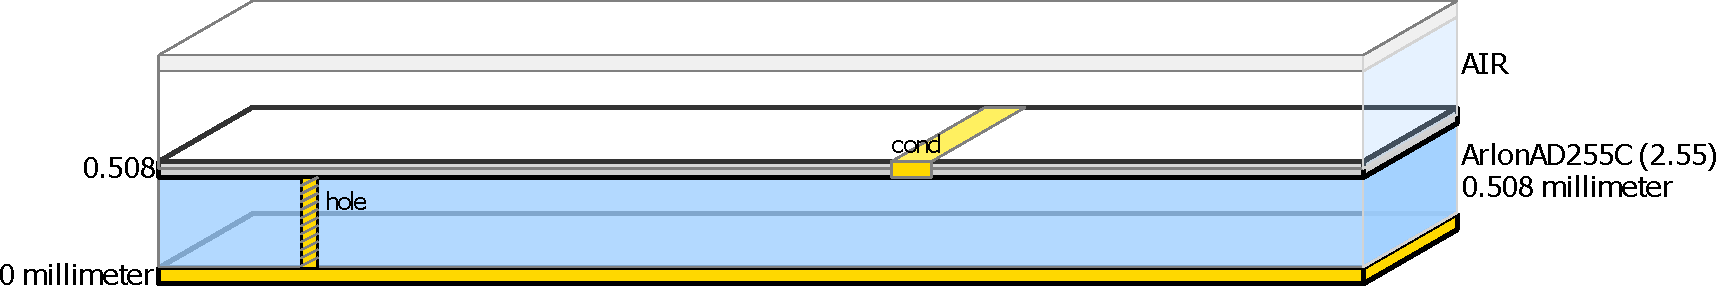
\includegraphics[width=0.9\textwidth]{wilk_divider_substrate.pdf}
    \caption{Подложка}%
    \label{fig:wilk_divider_substrate}
\end{figure}

\subsection{Модель на идеальных линиях передачи}

Соберём моделируемую схему на идеальных линиях передачи (Рис.~\ref{fig:wilk_divider_ideal_schematic}).

Результаты моделирования можно увидеть на рис.~\ref{fig:wilk_divider_ideal_data_1}.

\begin{figure}[!ht]
    \centering
    \begin{subfigure}[b]{0.50\textwidth}
        \centering
        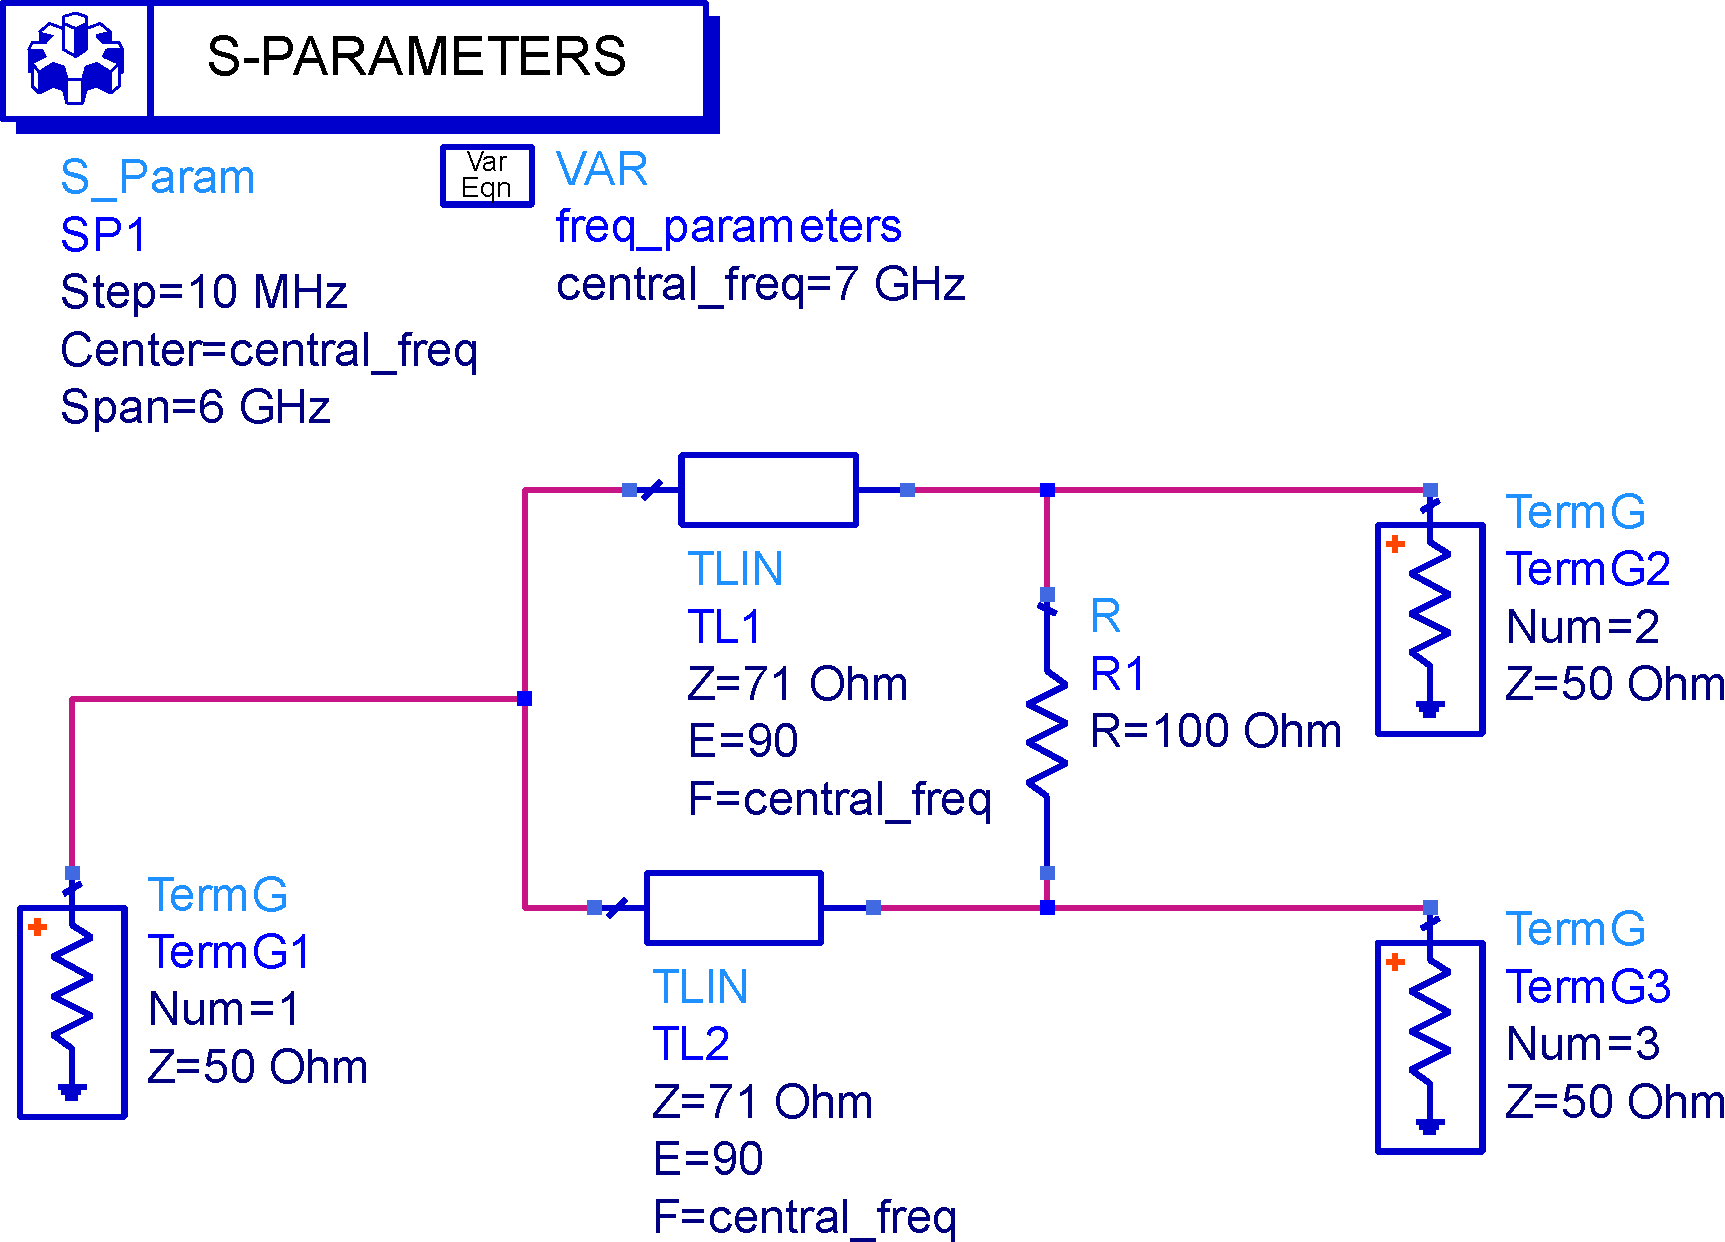
\includegraphics[width=\textwidth]{wilk_divider_ideal_schematic.pdf}
        \caption{}%
        \label{fig:wilk_divider_ideal_schematic}
    \end{subfigure}
    \hfill
    \begin{subfigure}[b]{0.40\textwidth}
        \centering
        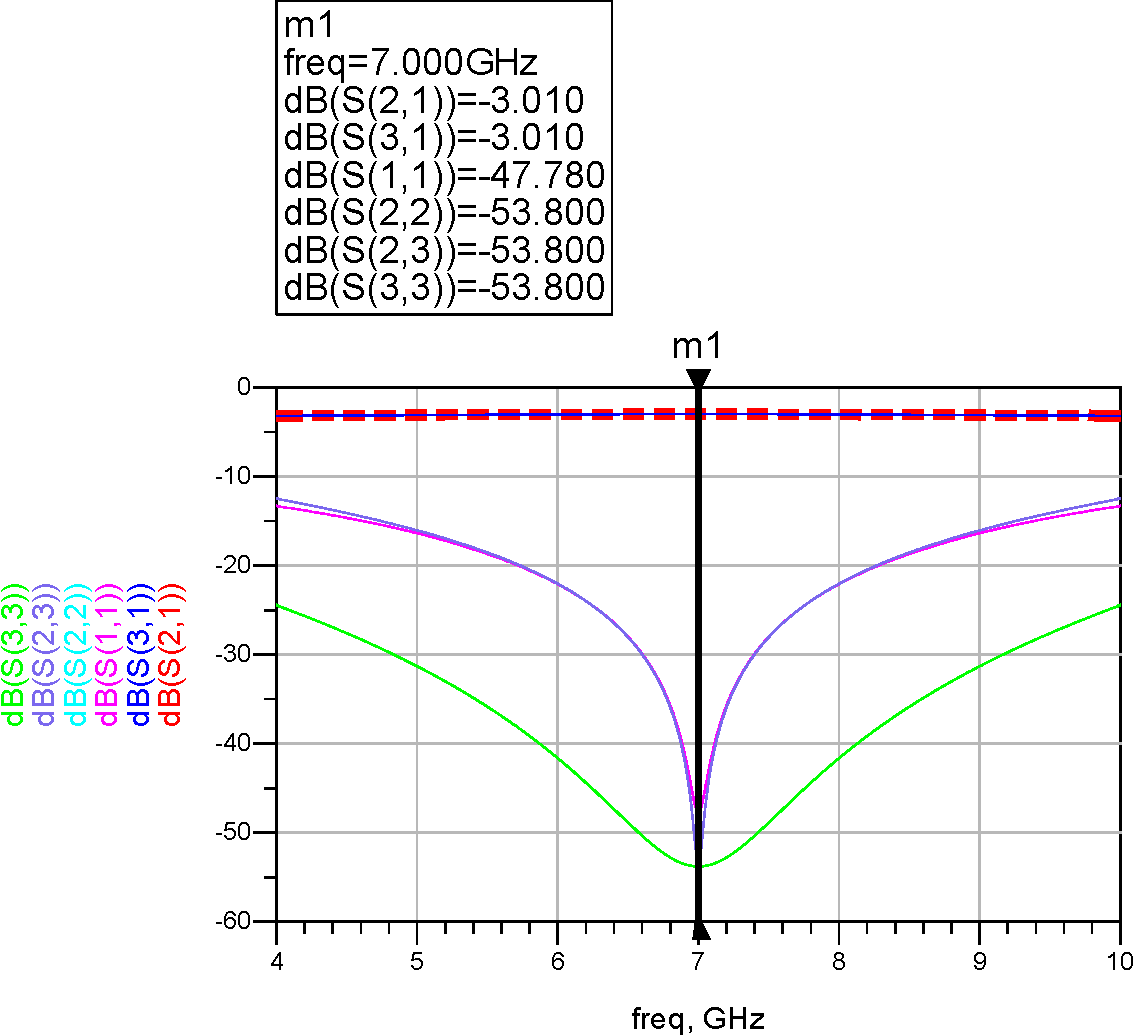
\includegraphics[width=\textwidth]{wilk_divider_ideal_data_freq_response.pdf}
        \caption{}%
        \label{fig:wilk_divider_ideal_data_freq_response}
    \end{subfigure}
    \caption{%
        (а) Моделируемая цепь на идеальных линиях передачи;
        (б) АЧХ моделируемой цепи
    }%
    \label{fig:wilk_divider_ideal_data_1}
\end{figure}

Выведем прямоугольный график с амплитудными соотношениями --- коэффициенты передачи из порта 1 в порты 2 и 3, развязку между 2 и 3.
Также отобразим на графике коэффициенты отражения от портов 1, 2 и 3.

Из графика видно, что
\begin{itemize}
    \item $dB(S_{21})$ и $dB(S_{31})$ полностью совпадают, т.к. каналы симметричны;
    \item моделируемая схема имеет хорошее согласование, т.к. коэффициенты отражения по всем портам не превышают $-40~\text{дБ}$;
    \item коэффициенты передачи из порта 1 в порты 2 и 3 близки к -3~дБ, т.е. устойство гибридное;
    \item развязка большая;
    \item устройство настроено точно на заданную частоту.
\end{itemize}

\subsection{Модель на схемном уровне в микрополосковом исполнении}

Для расчёта геометрических размеров нескольких видов линий передач воспользуемся инструментом LineCalc, которую можно найти по пути Tools \textrightarrow\ LineCalc \textrightarrow\ Start LineCalc.

В подокне Substrate Parameters задаём параметры подложки из технического задания, в подокне Component Parameters задаём частоту из технического задания, а в подокне Electrical --- импеданс и электрическую длину, для которых ведётся расчёт.
После этого, нажав кнопку Synthesize, получим в подокне Physical искомые геометрические размеры.

Расчитаем таким образом необходимые геометрические размеры отрезков.
Получим $W_{50} = 1.382~\text{мм}$ и $W_{71} = 0.755~\text{мм}$, $L_\text{71} = 7.535~\text{мм}$.

Электрические длины дуг проектируемого кольца имеют длину $\frac{\pi}{4}$, а геометрический угол равен $\pi$.
Пользуясь этим, поместим в блоке переменных выражение для расчёта радиуса дуг $R = \frac{L_{71}}{2 \pi} \cdot \frac{2 \pi}{\pi}$.

Осталось учесть только размеры резистора и отводящих линий.
В качестве резистора будем использовать SMD-резистор.
В моделируемой цепи подходящим вариантом будет SMD-резистор типоразмера 1206 со следующими геометрическими размерами: длина $L_\text{res} = 3.1~\text{мм}$, длина выводов $S_\text{res} = 0.5~\text{мм}$ и ширина выводов $W_\text{res} = 1.6~\text{мм}$.

Для компенсации длины резистора и выводящих линий будем использовать два участка МПЛ шириной $W_{71}$ и длиной $L_\text{add} = \frac{1}{2} (L_\text{res} + W_{50})$.

Со стороны первого порта поставим МПЛ шириной $W_{50}$ и длиной $L_\text{feed} = 1.5~\text{мм}$, а со стороны второго и третьего портов отводящие линии сделаем с помощью дуг шириной $W_{50}$, длиной в $\frac{\pi}{4}$ и радиусом $4 W_{50}$.

Построим моделируемую схему в микрополосковом исполнении (Рис.~\ref{fig:wilk_divider_MLIN_schematic_1}), после чего запустим расчёт и выведем АЧХ (Рис.~\ref{fig:wilk_divider_MLIN_data_1_response}).

\begin{figure}[!ht]
    \centering
    \begin{subfigure}[b]{0.45\textwidth}
        \centering
        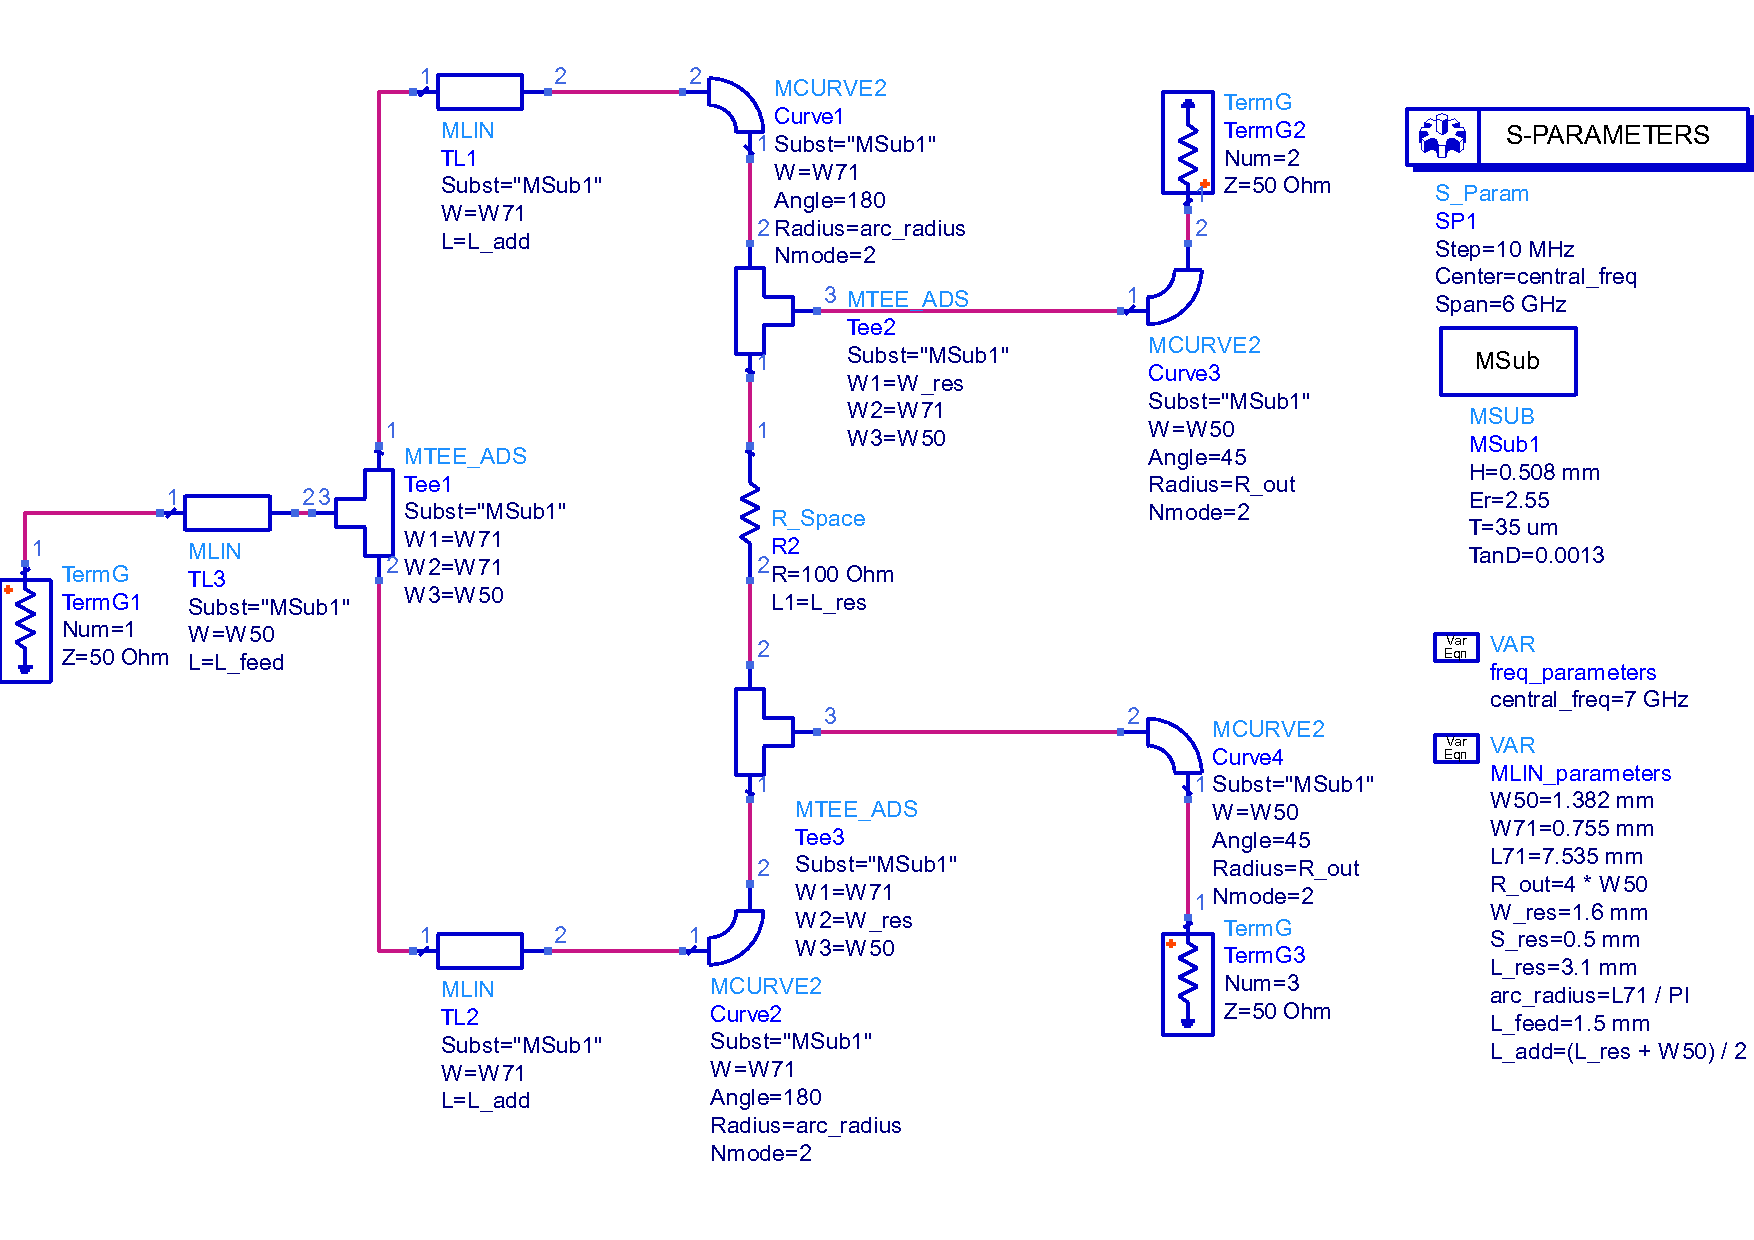
\includegraphics[width=\textwidth]{wilk_divider_MLIN_schematic_1.pdf}
        \caption{}%
        \label{fig:wilk_divider_MLIN_schematic_1}
    \end{subfigure}
    \hfill
    \begin{subfigure}[b]{0.45\textwidth}
        \centering
        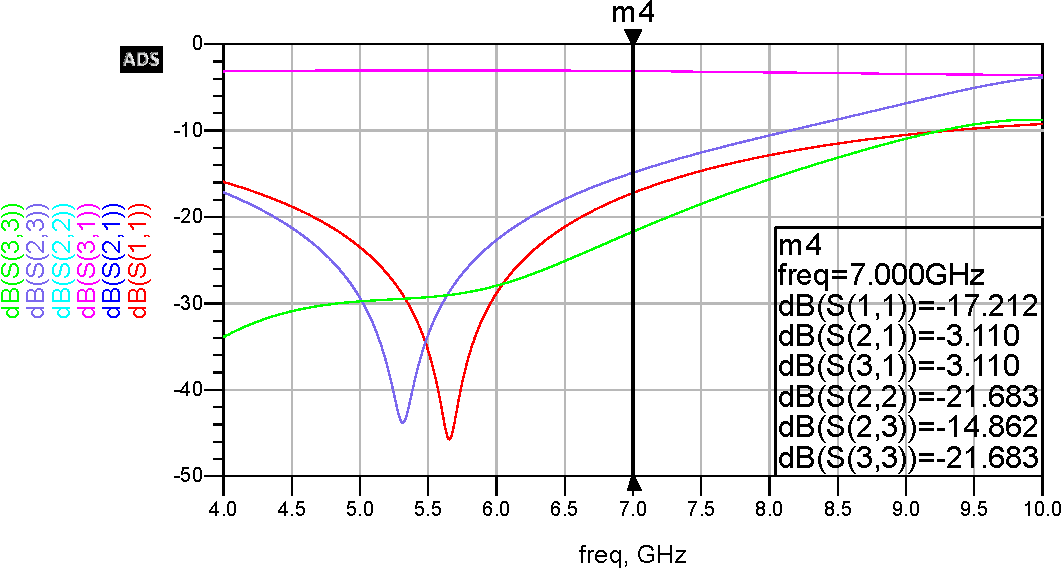
\includegraphics[width=\textwidth]{wilk_divider_MLIN_data_1_freq_response.pdf}
        \caption{}%
        \label{fig:wilk_divider_MLIN_data_1_freq_response}
    \end{subfigure}
    \caption{%
        (а) Моделируемая схема в микрополосковом исполнении;
        (б) АЧХ моделируемой цепи
    }%
    \label{fig:wilk_divider_MLIN}
\end{figure}

Результаты показывают, что рабочая частота устройства уплыла вниз.
Это связано с тем, что электические длины дуг превысили необходимые значения из-за того, что были добавлены тройники и компенсирующие их участки.

Для того чтобы исправить это, воспользуемся инструментом Tune.
В качестве регулируемого параметра укажем $L_{71}$, т.к. от него зависит радиус дуг.
Итоговый вид схемы представлен на рис.~\ref{fig:wilk_divider_MLIN_schematic_2}, а её характеристики на рис.~\ref{fig:wilk_divider_MLIN_data_2_freq_response}.

\begin{figure}[!ht]
    \begin{subfigure}[!ht]{0.45\textwidth}
        \centering
        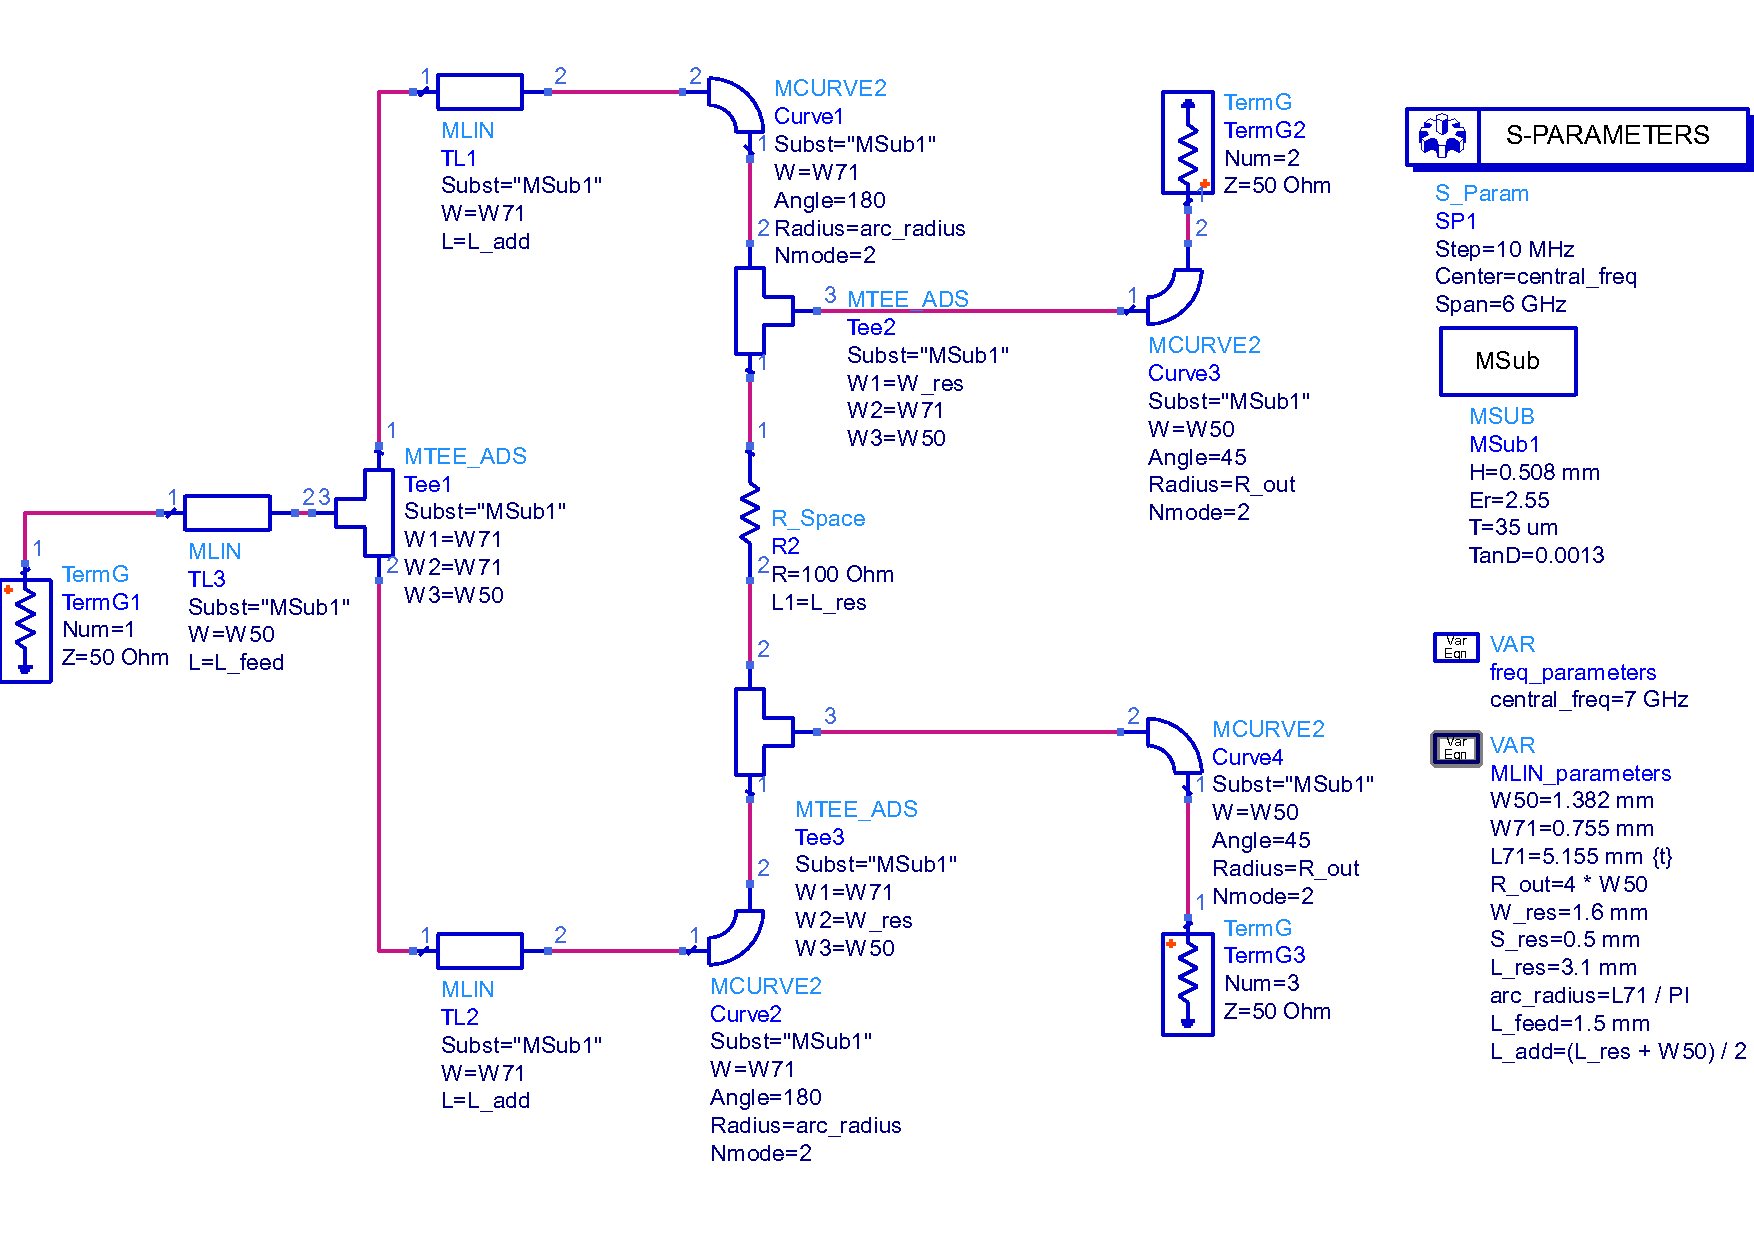
\includegraphics[width=\textwidth]{wilk_divider_MLIN_schematic_2.pdf}
        \caption{}%
        \label{fig:wilk_divider_MLIN_schematic_2}
    \end{subfigure}
    \hfill
    \begin{subfigure}[!ht]{0.45\textwidth}
        \centering
        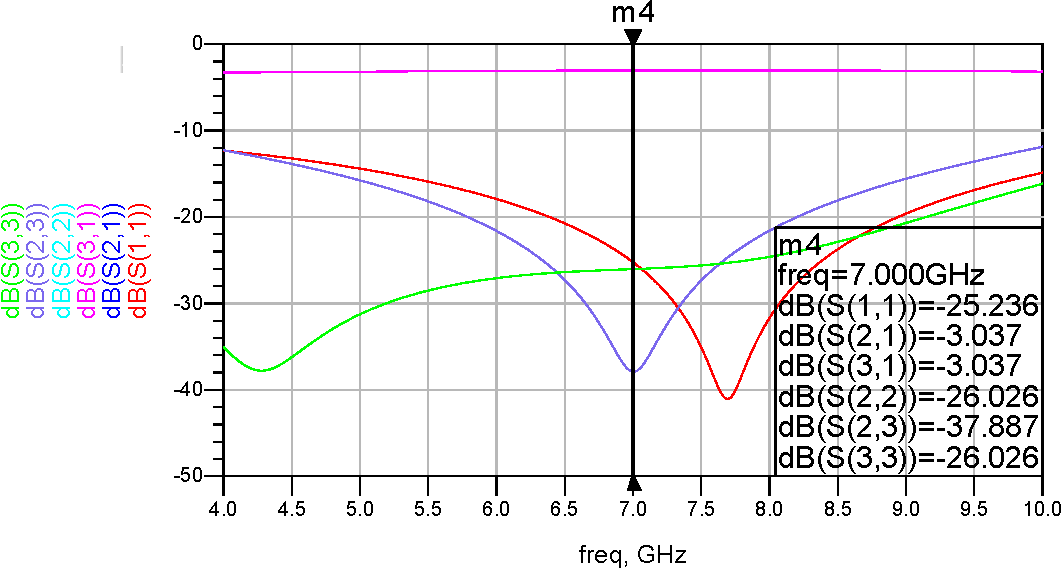
\includegraphics[width=\textwidth]{wilk_divider_MLIN_data_2_freq_response.pdf}
        \caption{}%
        \label{fig:wilk_divider_MLIN_data_2_freq_response}
    \end{subfigure}
    \caption{%
        (а) Моделируемая схема в микрополосковом исполнении;
        (б) АЧХ моделируемой цепи
    }%
    \label{fig:wilk_divider_MLIN_tuned}
\end{figure}

Оценим свойства схемы в отрезке частот $\pm 1.2~\text{ГГц}$ (Рис.~\ref{fig:wilk_divider_MLIN_data_2_freq_response_band}).

\begin{figure}[!ht]
    \centering
    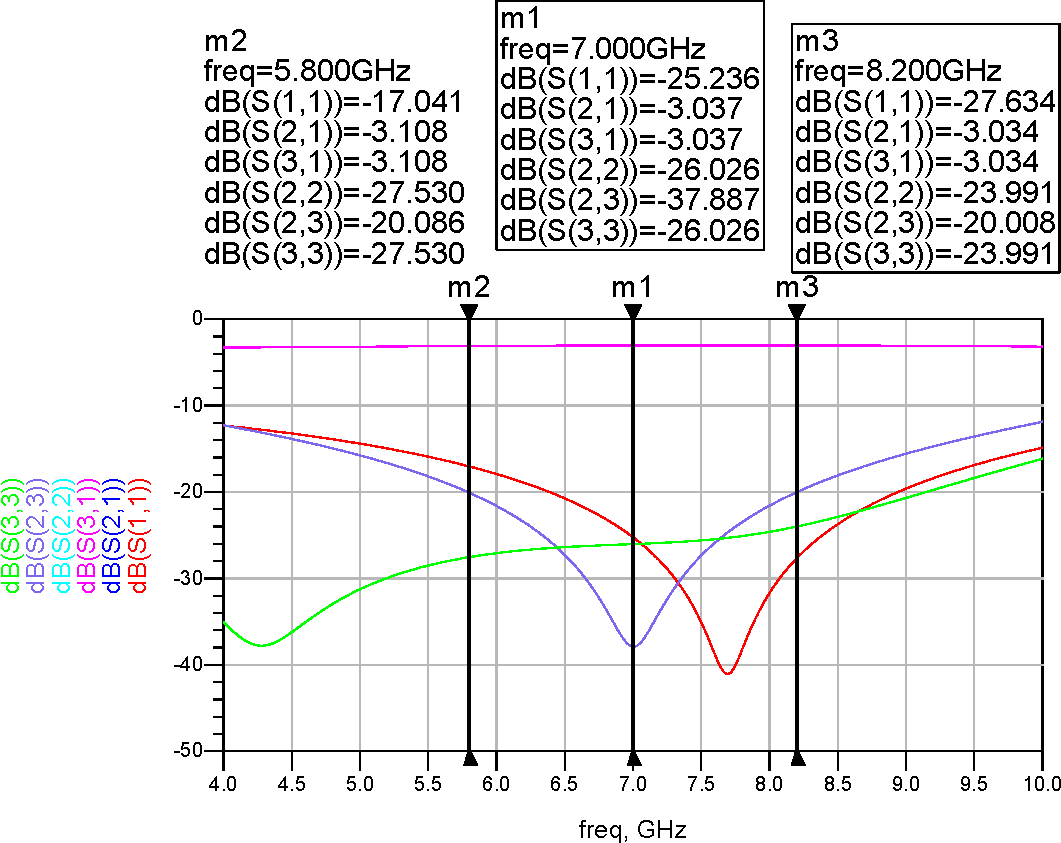
\includegraphics[width=0.8\textwidth]{wilk_divider_MLIN_data_2_freq_response_band.pdf}
    \caption{АЧХ моделируемой цепи}%
    \label{fig:wilk_divider_MLIN_data_2_freq_response_band}
\end{figure}

Из выведенных соотношений можно сделать следующие выводы:
\begin{itemize}
    \item устройство является гибридным во всей заданной полосе, т.к. $dB(S_{21})$ и $dB(S_{31})$ близки к -3~дБ;
    \item развязка $dB(S_{23})$ во всей полосе не превышает -20~дБ;
    \item коэффициент отражения $dB(S_{11})$ во всей полосе не превышает -17~дБ;
    \item коэффициенты отражения $dB(S_{22})$ и $dB(S_{23})$ сохраняется в пределах -20~дБ;
\end{itemize}

\subsection{Модель на топологическом уровне}

Скопируем схему в микрополосковом исполнении в новую ячейку. Сделаем её двухуровневой, перенеся во внутренний уровень все полосковые устройства. Сделать это можно по команде Edit \textrightarrow\ Component \textrightarrow\ Create Hierarchy.

В результате получим схему верхнего уровня (Рис.~\ref{fig:wilk_divider_EM_schematic_1}) и схему нижнего уровня (Рис.~\ref{fig:wilk_divider_EM_inner_schematic}).

\begin{figure}[!ht]
    \centering
    \begin{subfigure}[b]{0.55\textwidth}
        \centering
        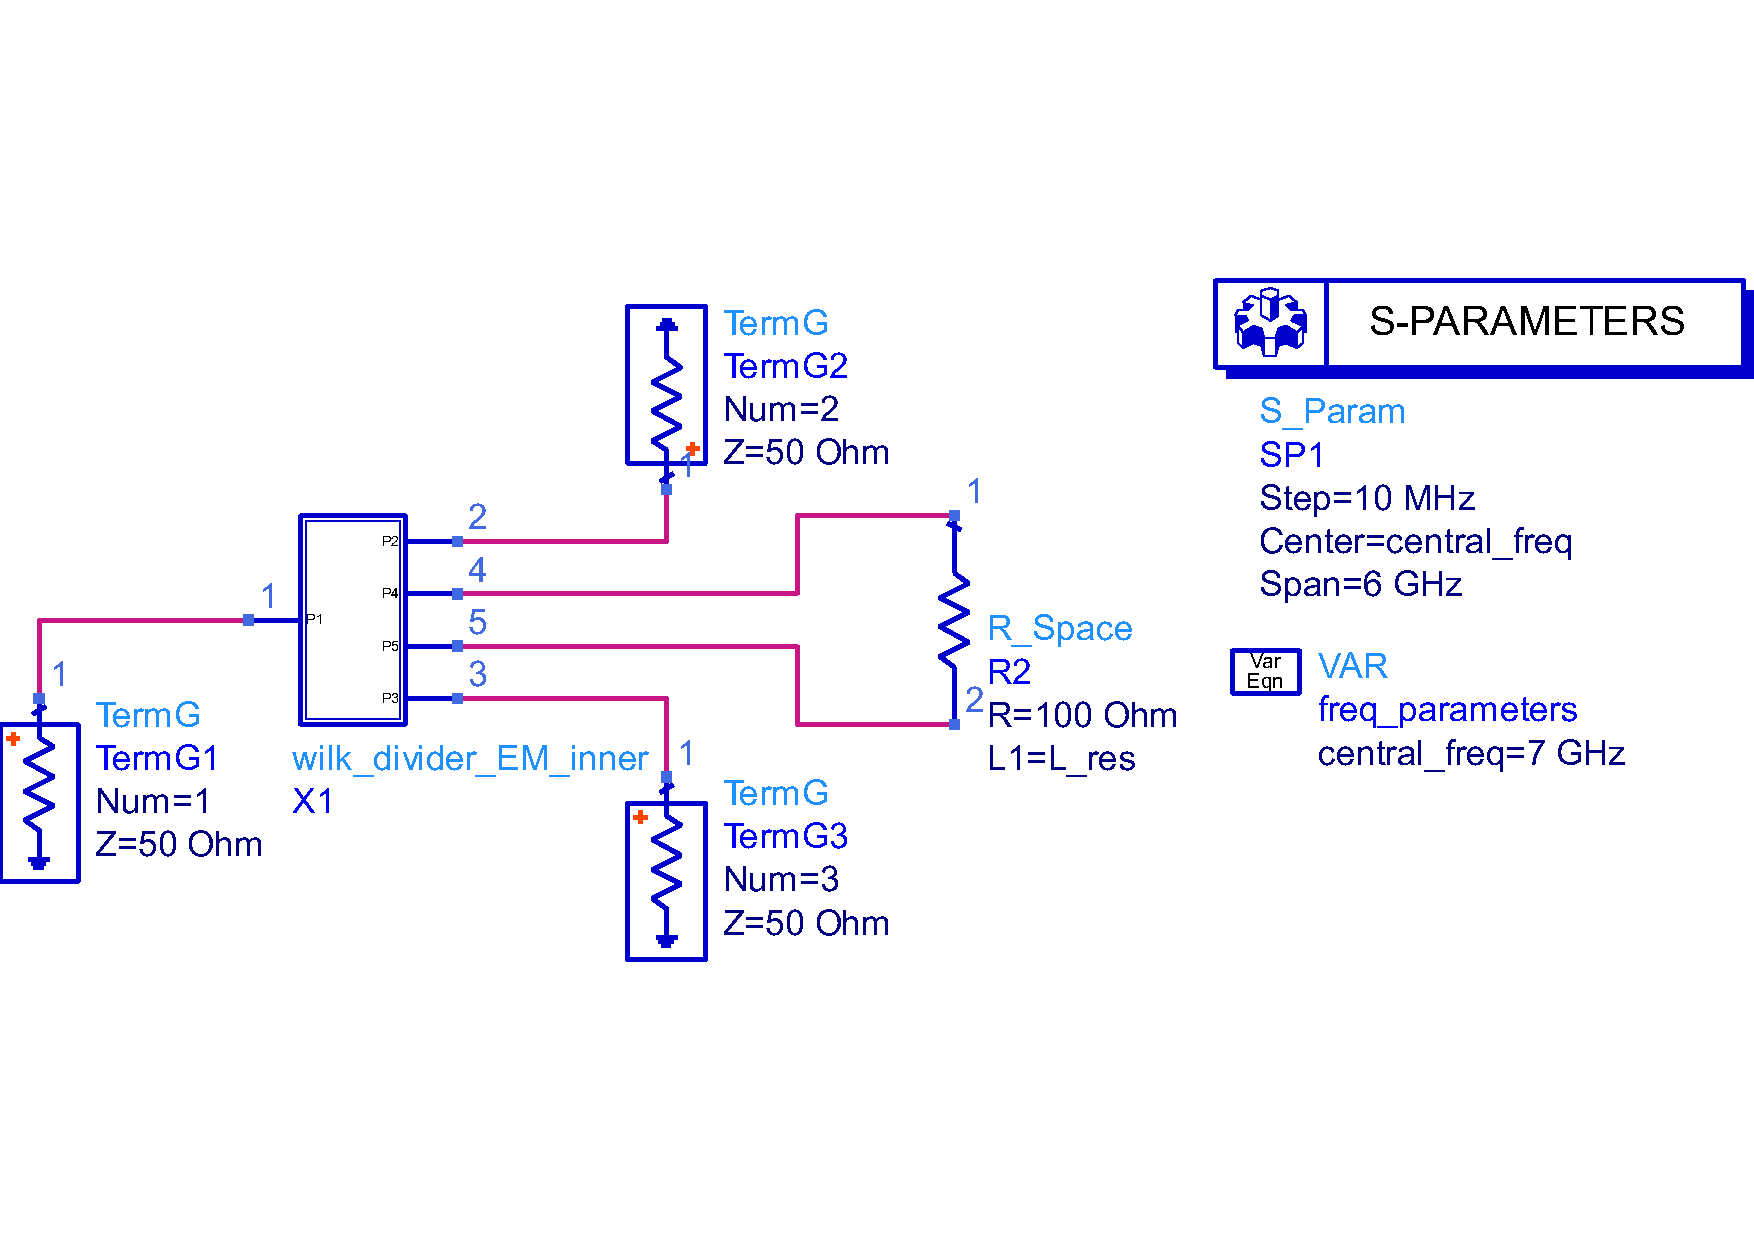
\includegraphics[width=\textwidth]{wilk_divider_EM_schematic_1.pdf}
        \caption{}%
    \label{fig:wilk_divider_EM_schematic_1}
    \end{subfigure}
    \hfill
    \begin{subfigure}[b]{0.35\textwidth}
        \centering
        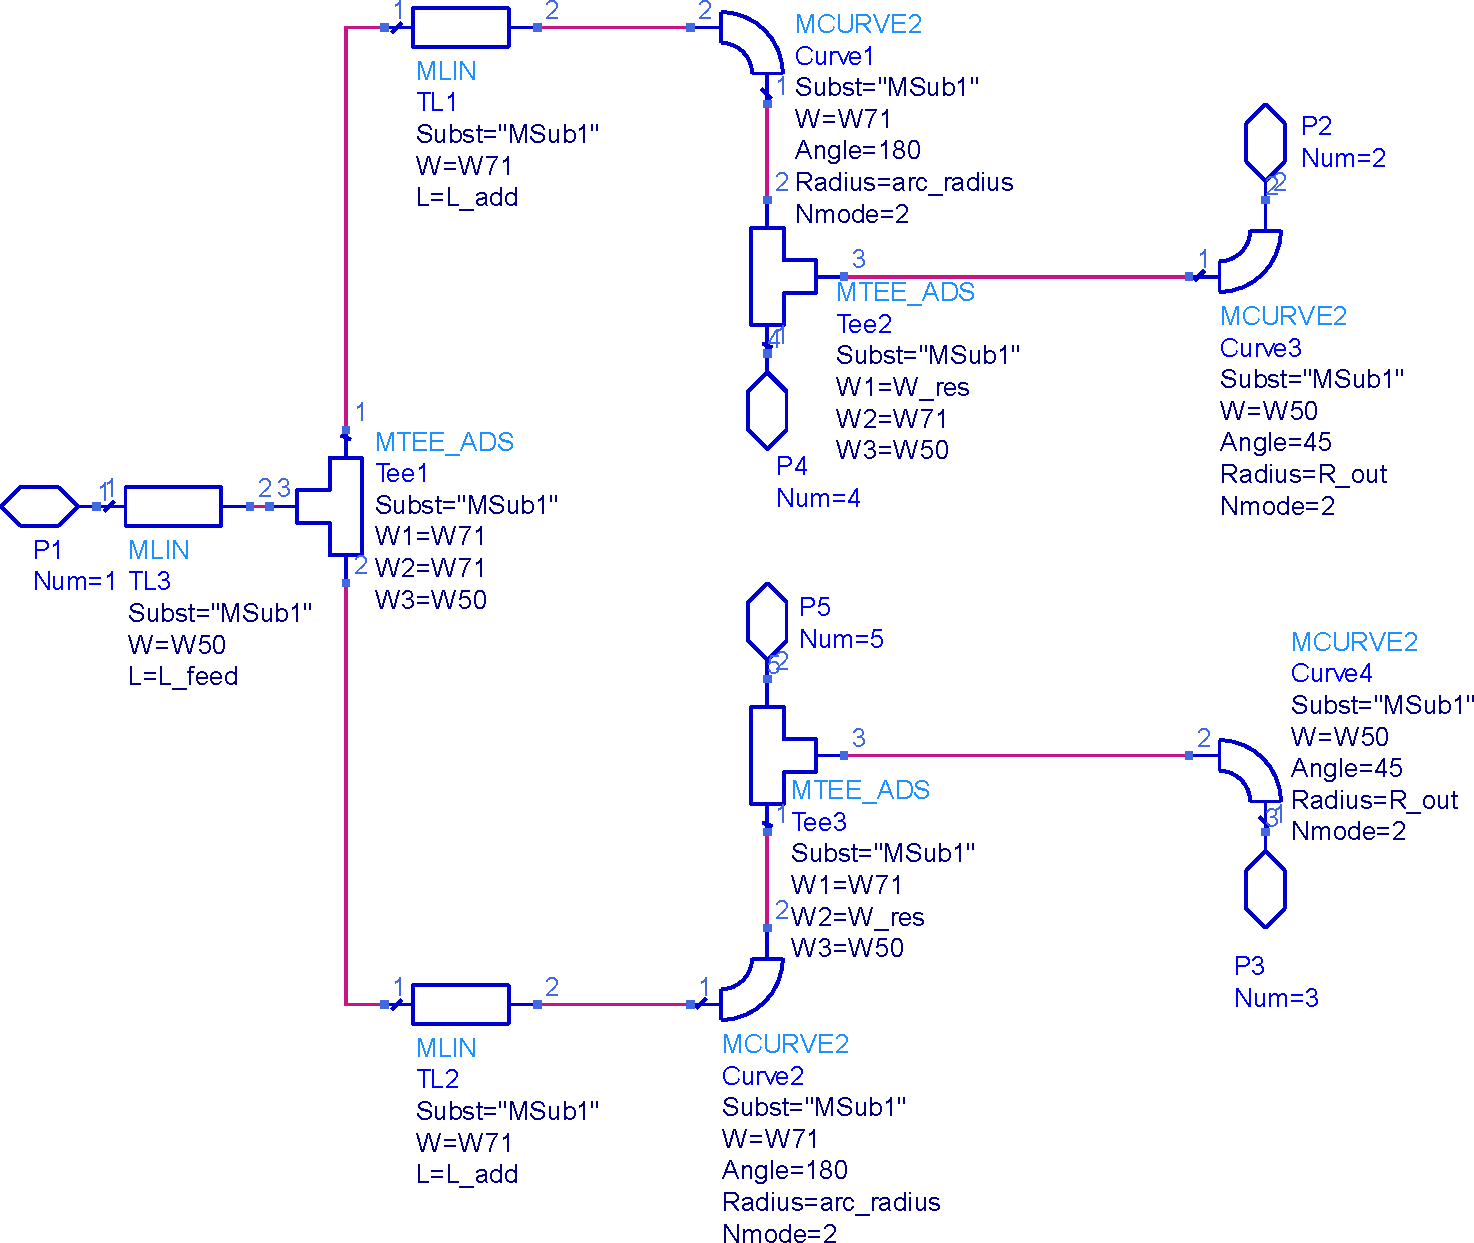
\includegraphics[width=\textwidth]{wilk_divider_EM_inner_schematic.pdf}
        \caption{}%
    \label{fig:wilk_divider_EM_inner_schematic}
    \end{subfigure}
    \caption{%
        Моделируемая схема на топологическом уровне:
        (a) внешнаяя схема;
        (б) внутренняя схема
    }%
    \label{fig:wilk_divider_EM_schematics}
\end{figure}

Перейдём в схему нижнего уровня. Для получения топологического представления воспользуемся функцией Layout \textrightarrow\ Generate/Update Layout.

\begin{wrapfigure}{l}{0.2\textwidth}
    \centering
    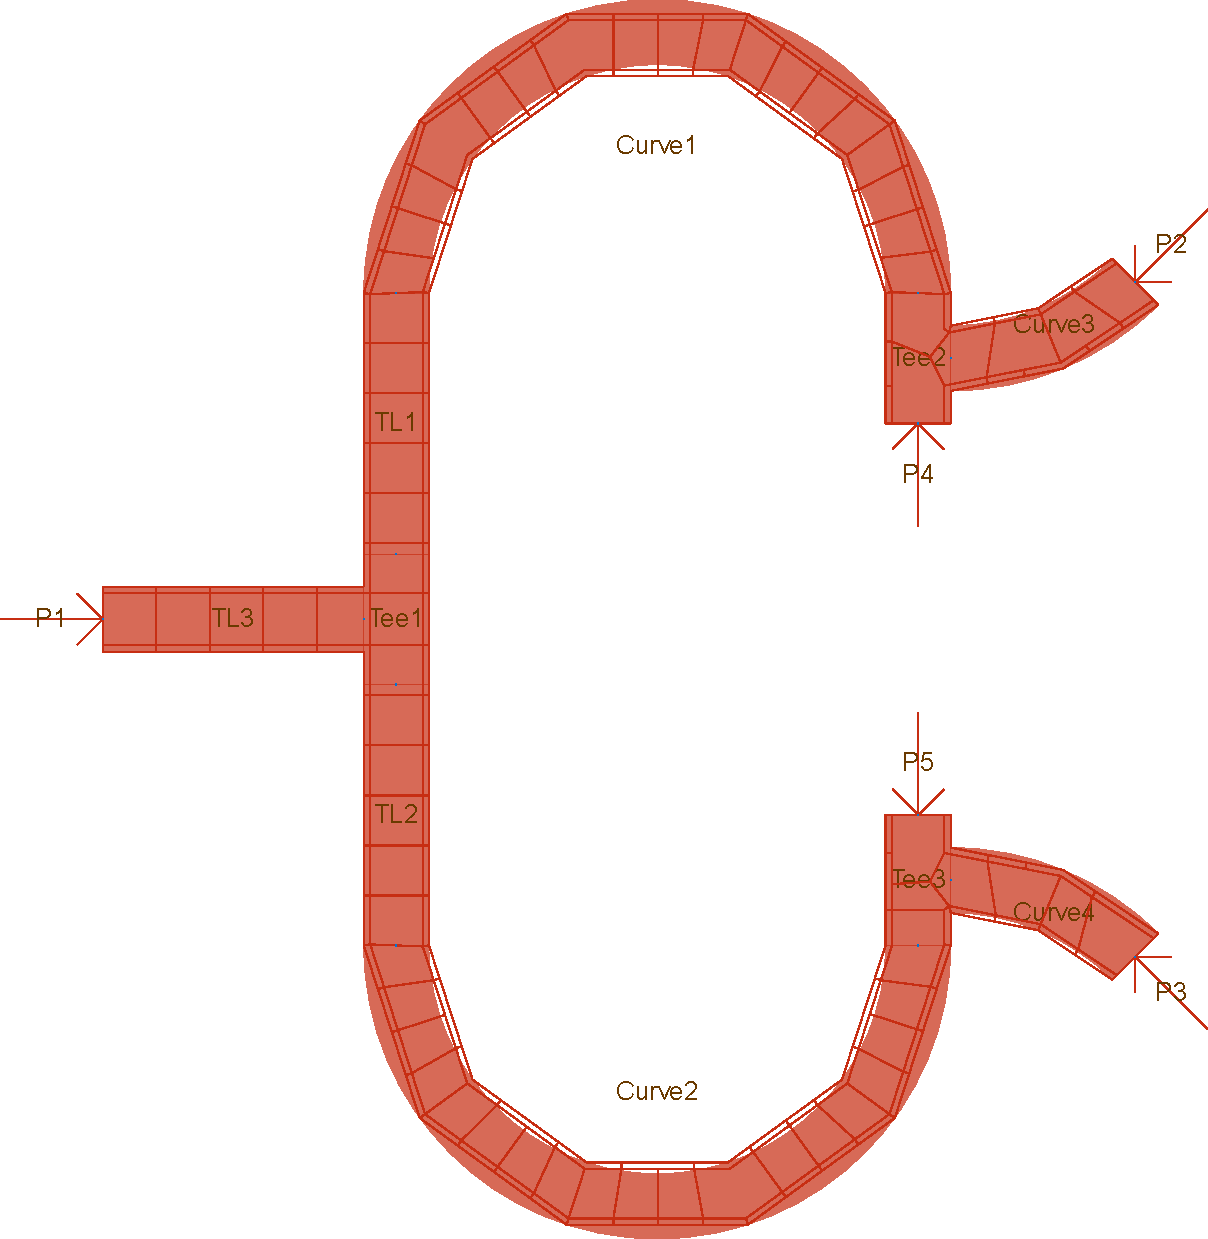
\includegraphics[width=0.2\textwidth]{wilk_divider_layout_sparam.pdf}
    \caption{Топологическое представление после проведения EM-моделирования}%
    \label{fig:wilk_divider_layout_sparam}
\end{wrapfigure}
Перейдём в окно File \textrightarrow\ Customize Pcell.
Сделаем схему параметризуемой, выбрав в выпадающем списке тип Parameterized sub network Pcell.
Также убедимся в том, что выставлены галочки напротив Support non-90 degree rotation и Support unit and database resolution for ADS 2015 and older.

В окне File \textrightarrow\ Cell Parameters определим параметры $W_{50}$, $W_{71}$ и прочие.

Для EM-моделирования создадим сущность emSetup.
Это можно сделать в окне EM \textrightarrow\ Simulation Setting.
Определим параметры в соответствии с требованиями.

Запустим EM-моделирование нажатием кнопки Simulate.
В результате на топологии появится сетка (Рис.~\ref{fig:wilk_divider_layout_sparam}).

Из окна emSetup можно обновить отображение элемента на схеме.
Сделаем так, чтоб оно подгружалось из топологии.
В итоге схема приобретёт вид как на рис.~\ref{fig:wilk_divider_EM_schematic_2}.

\begin{figure}[!ht]
    \centering
    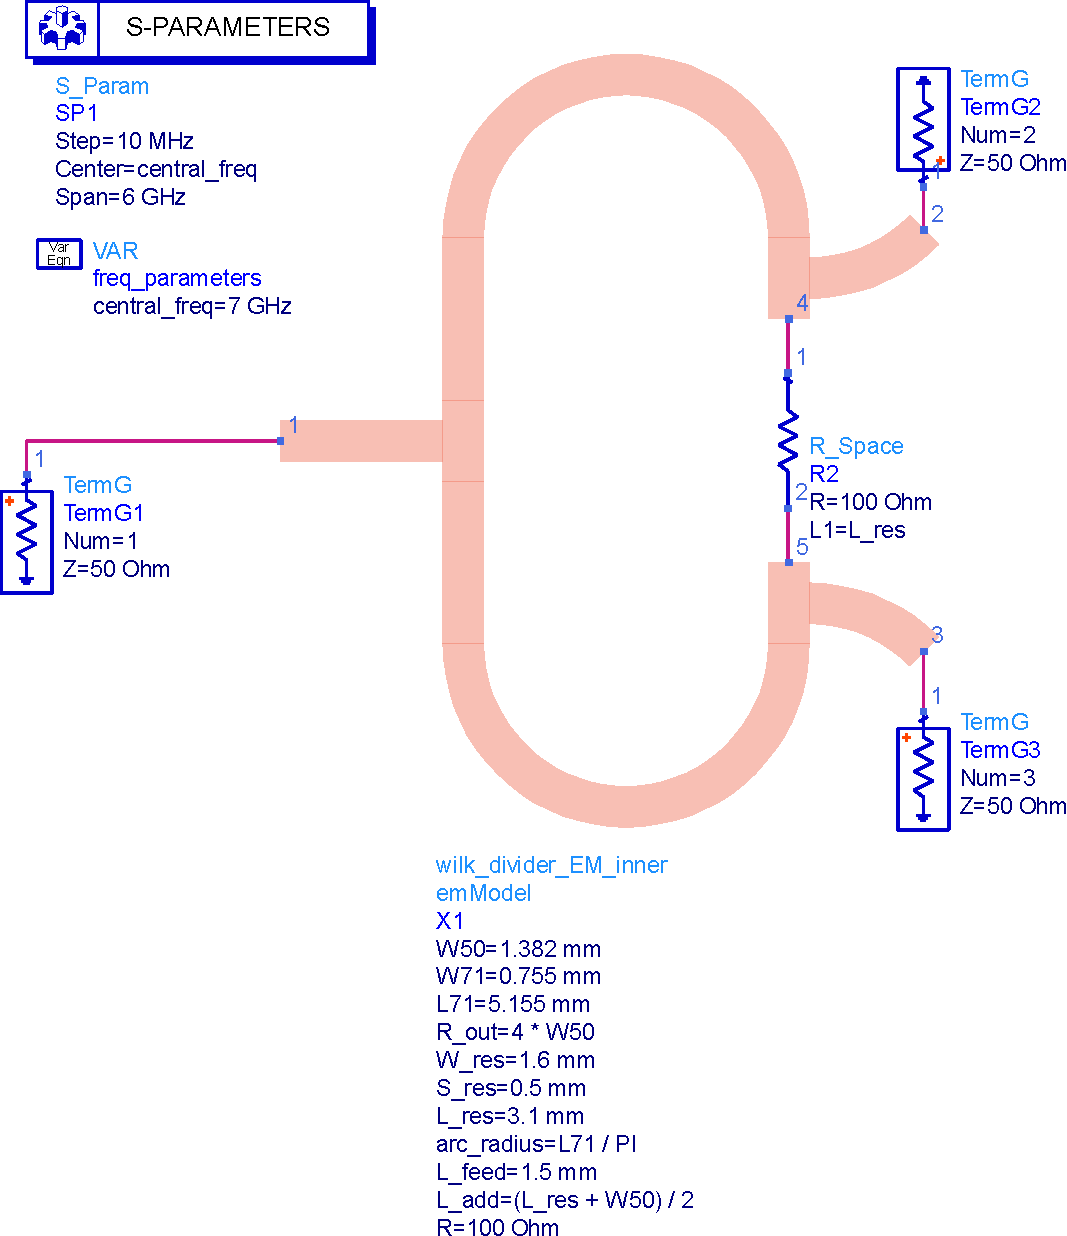
\includegraphics[width=0.6\textwidth]{wilk_divider_EM_schematic_2.pdf}
    \caption{Итоговый вид схемы}%
    \label{fig:wilk_divider_EM_schematic_2}
\end{figure}

Запустим моделирование и отобразим частотные характеристики (Рис.~\ref{fig:wilk_divider_EM_data_1_freq_response}).

\begin{figure}[!ht]
    \centering
    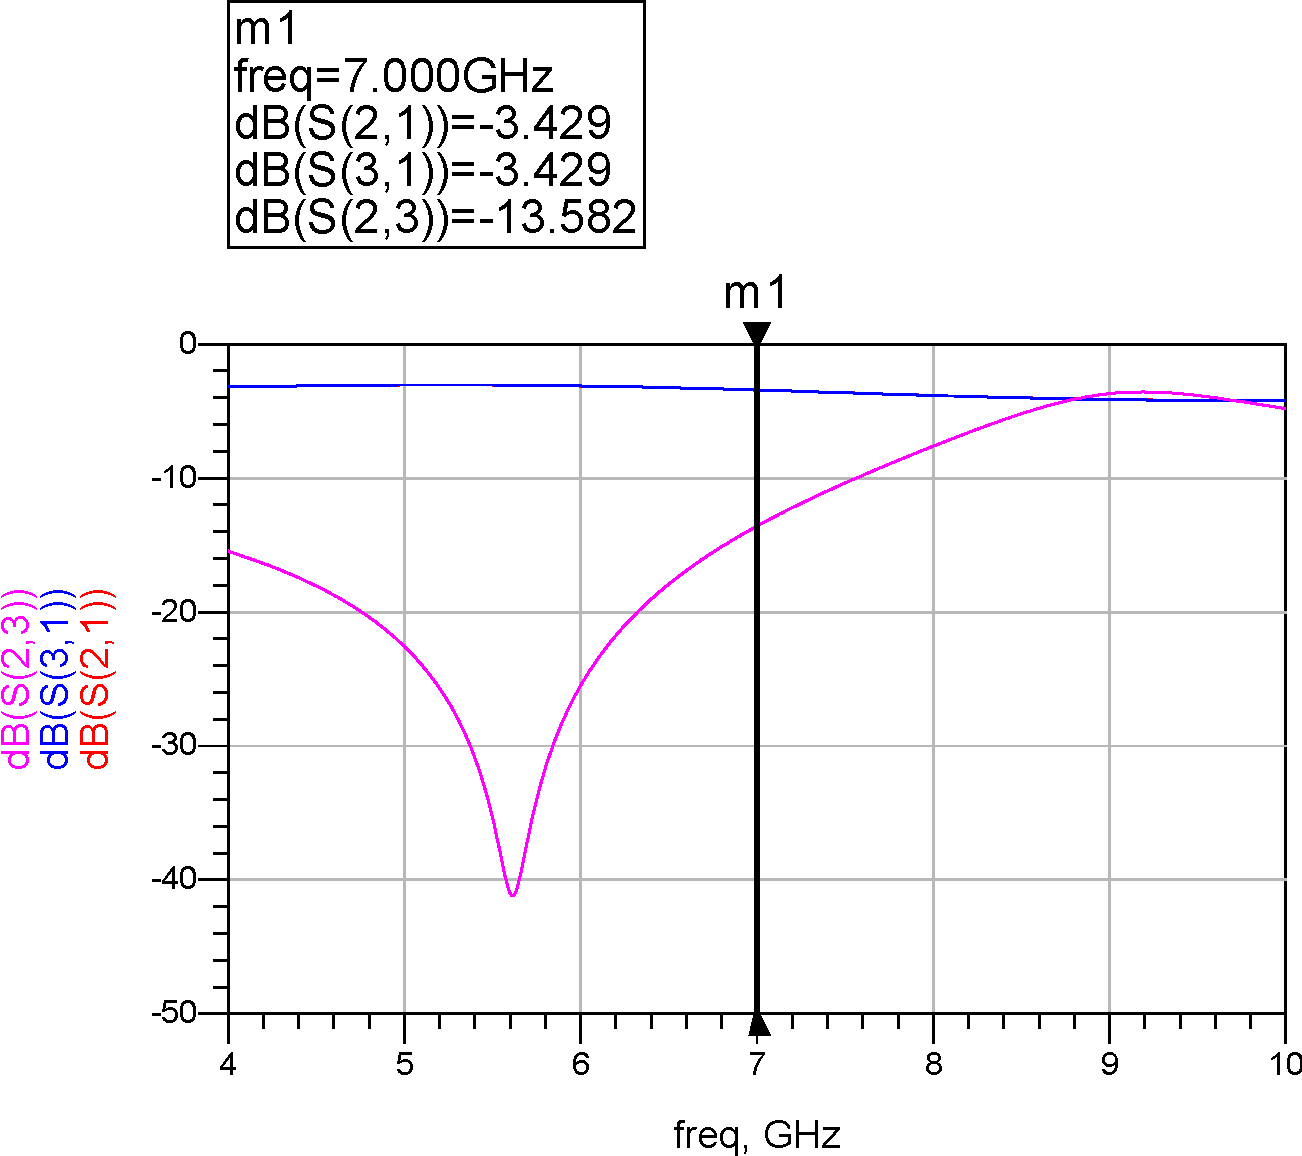
\includegraphics[width=0.7\textwidth]{wilk_divider_EM_data_1_freq_response.pdf}
    \caption{АЧХ моделируемой схемы в топологическом представлении}%
    \label{fig:wilk_divider_EM_data_1_freq_response}
\end{figure}

Рабочая частота уплыла.
Исправим это подгонкой параметров.
Результат представлен на рис.~\ref{fig:wilk_divider_EM_data_2_freq_response}.

\begin{figure}[!ht]
    \centering
    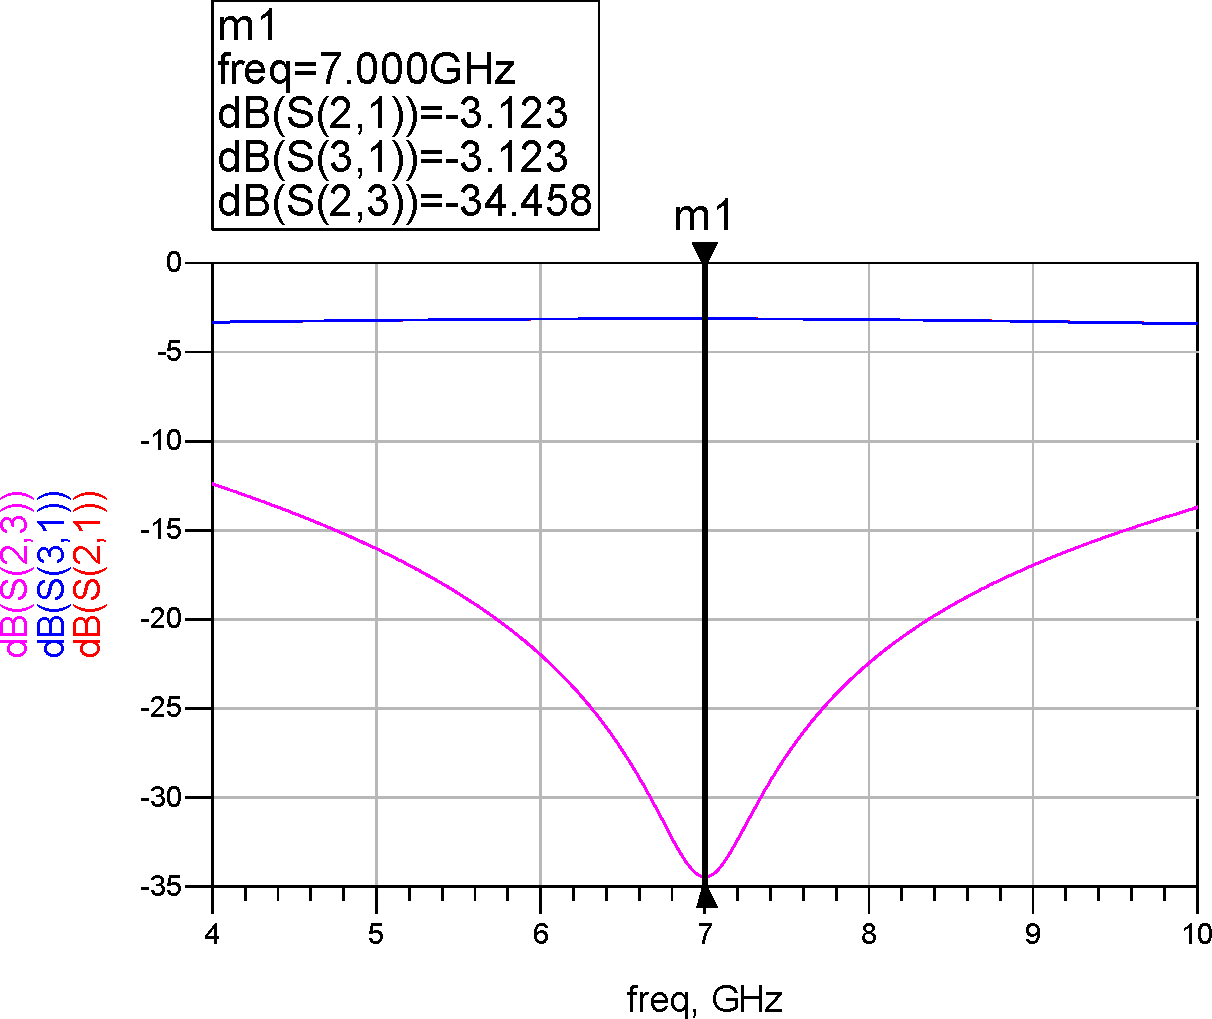
\includegraphics[width=0.7\textwidth]{wilk_divider_EM_data_2_freq_response.pdf}
    \caption{АЧХ моделируемой схемы в топологическом представлении}%
    \label{fig:wilk_divider_EM_data_2_freq_response}
\end{figure}
